\title{Implementing pseudonym based approach to secure the long-term-identity privacy of mobile users using 5G enabled mobile-phones, home-networks along with legacy serving-networks and USIMs}
\author{
        Khan, Niemi, Akman\\
        Department of Computer Science\\
        University Of Helsinki\\
        Helsinki, \underline{Finland}
}
\date{\today}

\documentclass[12pt]{article}
\usepackage[]{xcolor}
\usepackage{amsfonts}
\usepackage[]{amsmath}
\usepackage{graphicx}
\usepackage{eqnarray}



\begin{document}
\maketitle



\begin{abstract}
To secure the privacy of long term identity of mobile phone users, recently two different approaches have been published. One is the use of pseudonyms and the other is the use of public-key cryptography where the public-private key pair is owned by the home network (HN). In this article, the challenges which will come forward while implementing those two approaches are discussed. In some cases, plausible solutions are proposed.
\end{abstract}


\section*{Introduction}
An IMSI (Internation Mobile Subscriber Identity) which is the long term identity of a mobile phone subscriber is a string composed of 15 decimal digits. It has three parts: mobile country code (MCC), mobile network code(MNC), and mobile subscriber identification number (MSIN) where 
$$IMSI = MCC||MNC||MSIN$$ Pseudonym and public-key cryptography, in both of the approaches, the MCC and MNC are sent across the mobile network in clear text and focus on the privacy of MSIN part only. We will also focus on the same principle in this article and will mean the privacy of MSIN when we mention about the privacy of IMSI. Note that there are only $10$ decimal digits represented by $40$ binary bits available to represent an MSIN (\textcolor{red}{cite}).



\section*{The Pseudonym scheme}
\subsection*{Goals:}
\begin{enumerate}
        \item \label{goal_privacy} Privacy of the long-term-identity from any outsider and also from honest but curious insider by using a temporary identity of a user recognized by HN. This temporary identity is also called a pseudonym.
        \item  \label{goal_backward_compatibility} The scheme has to be compatible with the legacy USIMs and serving networks (SN) so that the scheme can be brought into use only by modifying the mobile equipment (ME) and HN.
        \item \label{goal_privacy_sn} Privacy of the pseudonym even from the SN. That is, the SN involved in an AKA will not know the pseudonym of a user which the user will use in another AKA when he moves to another SN.
\end{enumerate}  

\subsection*{The scheme:}
\begin{enumerate}
    \item \label{issue_initial_pseudonym} Every user having an IMSI is given a pseudonym $P$ by the HN initially.
    \item  When the user identifies itself with $P$ to the SN, the SN forwards $P$ to the HN
    \item \label{scheme_aka_step} In response, along with the authentication vector (AV) and pseudonym $P$, the home subscription server (HSS) in the HN sends a new pseudonym $P^{'}$ to the SN encrypted by the secret key $K$ or by some other secret key $P_{pseudo}$ derived from $K$.
    \item The SN runs the AKA with UE based on the AV it received from the SN. It also sends the encrypted new pseudonym $P^{'}$ to the UE.
    \item If the AKA is successful then the ME will be able to decrypt it and obtain $P^{'}$. The old pseudonym $P$ will be continued in use instead of IMSI until the UE tries to connect via another SN. 
    \item  When the UE tries to connect to the network via a new SN, the new SN has no knowledge about $P$. At this point instead of sending the IMSI, the UE identifies itself with $P^{'}$ which leads into a new AKA run in the similar fashion mentioned in step \ref{scheme_aka_step}
    \item Whenever a new AKA is run, the HN generates a new pseudonym $P^{''}$ in the similar fashion mention in step \ref{scheme_aka_step}, replaces $P$ with $P^{'}$ and $P^{'}$ with $P^{''}$
\end{enumerate}

\subsection*{The implementation issues:} 
Here we describe the issues of the above scheme that we found while implementing it:
\begin{enumerate}
 \item How the HN assigns the first pseudonym $P$ to a user is an implementation issue with the mentioned scheme. A pseudonym can't be assigned to a USIM because the scheme needs to be compatible with legacy USIMs to achieve the goal \ref{goal_backward_compatibility}. The scheme also can not assign a pseudonym to an ME because a user is not identified by the ME but by the USIM. Besides, many USIMs can be inserted in in and ME over it's lifetime.
 
 \item \label{issue_secret_key} The pseudonym $P^{'}$ can not be encrypted by the master key $K$ or some other key derived from $K$. Because in that case, the decryption has to happen in USIM as the ME doesn't know the master key $K$. But the scheme needs to be compatible with the legacy USIM and such decryption is not a functionality of the legacy USIMs. Also this secret key needs to be unknown by the SN to achieve the goal \ref{goal_privacy_sn}.

\item \label{issue_sn_modification} This scheme requires the modification in the legacy SNs, because the SN needs to be able to receive the encrypted pseudonyms and send them to the UEs. This is not acceptable because the scheme needs to be compatible with legacy SNs according to goal \ref{goal_backward_compatibility}.

\item Another issue with this scheme is,  every user is associated with an IMSI and two pseudonyms. These 3 distinct IMSI looking strings for one user create pressure in the space of valid IMSIs or pseudonyms. The size of this space is only $10^{10}$. This is because in the standard, IMSI is defined to be composed of decimal digits (\textcolor{red}{cite}) and there might have the existence of SNs which strictly check on this constraint to validate an IMSI. 

\item \label{issue_imsi_looking_pseudonyms} This is already mentioned in the original paper that the pseudonyms have to look like the original IMSI so that the scheme becomes compatible with the legacy SNs. But it doesn't discuss how to generate such pseudonyms which are uniformly distributed in the pseudonym space.

\item \label{issue_conflict} It needs to be ensured that the newly generated pseudonym is not already in use as an IMSI or a pseudonym for a different user in the HN.

\item \label{issue_synchronization} Another important issue is, how to ensure the synchronization of the pseudonyms in use for a user in between the ME, SN and HSS. Apparently, the HSS needs to know that the UE has been successful in the AKA before it updates the entry of that user with the new pseudonym. Indeed, otherwise the HN and UE will have different pseudonyms if the AKA fails. To ensure it, the SNs has to acknowledge the HNs about the result of the AKA. This is not the case with the legacy SNs. However, even if an acknowledgement mechanism is introduced in the upcoming 5G networks, the acknowledgment itself might be lost even when the AKA is successful. Based on this weakness we can mount an active attack to make the pseudonyms in HN and ME inconsistent by setting up a fake base station. Here we describe the attack: \begin{enumerate}
    \item The attacker sets up a fake base station impersonating a legitimate SN and asks for the long term identity of the user
    \item The user responds to the query by sending it's pseudonym
    \item The attacker sends the received pseudonym to a legitimate SN leading to run an AKA in between the legitimate SN and the attacker. This AKA will cause the HN of the victim to update the entry of the victim with a new pseudonym. On the other hand, the victim has no knowledge about this AKA or the new pseudonym that the HN has updated the victim's entry with in the HSS. As a result, the victim will not update the pseudonym in the ME. Which means the synchronization of the pseudonyms in between ME and HN is lost and all the consequent AKA will fail even when the victim tries to connect with a legitimate SN 
\end{enumerate}


\item \textcolor{blue}{Note that, in this scheme the current SN knows the pseudonym $P$ that the user used during the last AKA and the SN also keeps it stored and use in error messages of a failed AKA. This pseudonym $P$ is also used to page for the UE. It is possible that the pseudonym $P$ of a user $U_{1}$ in the old SN ($SN_{1}$) will be kept stored and not deleted even when the user has moved to another SN ($SN_{2}$). Now if $U_{1}$ participates in an AKA in $SN_{2}$ then the user's pseudonym will be updated in HN and $SN_{2}$. Now if some other user $U_{2}$ comes in $SN_{1}$ and run an AKA, there is a tiny probability that user $U_{2}$ will be assigned with the pseudonym $P$ by the HN. This will cause the $SN_{1}$ to have more than one entries with one pseudonym even though there is no such conflict in the HN.}


\item (\textcolor{red}{The scheme might have some issue with the handover process from one eNodeB to another eNodeB, or from one MME to another MME. This issue needs to be checked closely})



\end{enumerate}



\section*{Potential Solutions}
\subsection*{Solution to issue \ref{issue_initial_pseudonym}:} Apparently there is no solution to the issue \ref{issue_initial_pseudonym} that uses a pseudonym and still works with the legacy USIMs. This leaves the only option of using the IMSI for the very first time. Fortunately using IMSI in such a manner still gives us the benefit of using a pseudonym. Because, using this IMSI, only for the very first time, and never after, makes the IMSI effectively a pseudonym itself. Besides, in a situation of such a limited use of the IMSI, an attacker interested in the IMSI of a target user has to eavesdrop on the target's AKA messages exactly at the very first time the target connects to the network. 
\subsection*{Solution to issue \ref{issue_secret_key}:}  To solve the issue \ref{issue_secret_key}, the secret key used for encrypting the new pseudonym $P^{'}$ can be CK, or IK, or generated from either one or both of them. This will work if the SN is of LTE. However, this solution fails to achieve the goal \ref{goal_privacy_sn} if the SN is of UMTS. Because CK and IK are known by an SN of UMTS.

\subsection*{Solution to issue \ref{issue_sn_modification}:}  One solution to the issue \ref{issue_sn_modification} could be to send the encrypted pseudonym as part of the RAND of AV. But there is a chicken-egg problem here. The keys CK and IK are derived from RAND. So, if the RAND includes the encrypted pseudonym then we need to know the CK and IK first. That is, we can't generate CK and IK without knowing RAND and we can't have RAND without knowing CK and IK. Figure \ref{fig:chicken-egg} shows the situation pictorially. To Solve the chicken-egg problem, we propose to generate the pseudonym $P^{'}$ separately both in HSS and ME end by encrypting the RAND which will be sent from HSS to SN as part of the AV in anyway. Our idea is to use keyed message authentication code (MAC) of the RAND to use as the pseudonym  $P^{'}$. 

  \begin{figure}[h!]
    \centering
    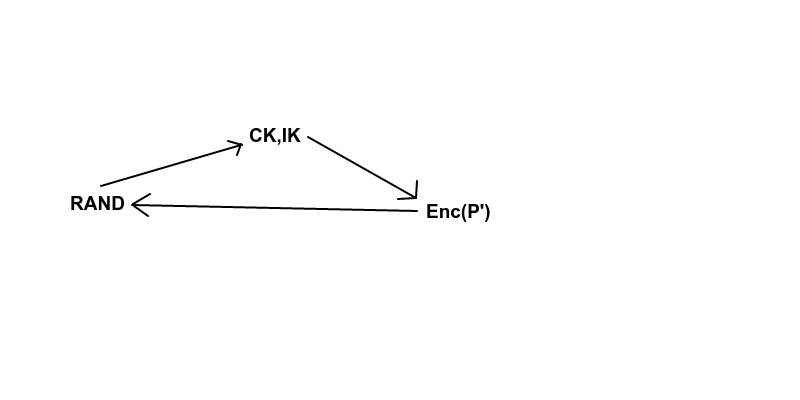
\includegraphics[width=0.7\textwidth , height = 5cm]{chicken-egg}
    \caption{The chicken-egg problem}
    \label{fig:chicken-egg}
    \end{figure}


\subsection*{Solution to issue \ref{issue_imsi_looking_pseudonyms} and \ref{issue_conflict}:} To solve the issues \ref{issue_imsi_looking_pseudonyms} and \ref{issue_conflict}, we have a proposal here:
    \begin{enumerate}
    \item Choose $RAND$ in the HSS using a random number gnerator. (\textcolor{red}{Use the same random number generator that is used in the existing HSSs})
    \item Generate CK and IK from the RAND. (\textcolor{red}{Use the same mechanism which is used in LTE})
    \item Generate a message authentication code (MAC) of $RAND$ using a key generated from $CK$ and $IK$  (\textcolor{red}{An appropriate HMAC has to be chosen})
    \item Lets say the MAC is $M = a_1 \cdots a_n$ where $a_i$ is the $i$-th bit of the code
    \item Let us represent $M$ as a sequence of $m$ hexadecimal digits, that is $M = a_1 \cdots a_n = h_1 \cdots h_{m}$ where $m = n/4$ and $h_{i}$ is the hexadecimal value represented by the bit string $$a_{(i-1)*4+1}a_{(i-1)*4+2}a_{(i-1)*4+3}a_{(i-1)*4+4}$$ 
    \item Consider a function $f:\mathbb{Z}_{15} \times \mathbb{Z}_2 \rightarrow \mathbb{Z}_{10}$ where 
\[
    f(h_i,a_n)= 
\begin{cases}
    h_i,& \text{if } 0\leq h_i\leq 9\\
    0+a_n,              & \text{if } h_i = A\\
    2+a_n,              & \text{if } h_i = B\\
    4+a_n,              & \text{if } h_i = C\\
    6+a_n,              & \text{if } h_i = D\\
    8+a_n,              & \text{if } h_i = E
\end{cases}
\]
    \item For every $i$, if $h_i$ is not equal to $F$, compute $d_i = f(h_i,a_n)$ until $10$ $d_i$s are obtained. If more or equal to $(m-9)$ $h_i$s are $F$, then go  back to step 1.
    \item The pseudonym is constructed by concatenating the $10$ $d_i$s in the same sequence they were were obtained.
    \item If the resultant pseudonym is already used as a pseudonym of IMSI, then go back to step 1 (\textcolor{red}{An appropriate data structure needs to be chosen to make this search less expensive})
    \end{enumerate}
    %Note that, with this solution, the HN doesn't need to store two pseudonyms $P$ and $P^{'}$. It can store only the pseudonym $P$ and whenever an AKA is run, it generates $P^{'}$ and update $P$ with the generated $P^{'}$. \paragraph{}
    
    One issue with the above approach is, the HSS might end up in generating shorter or duplicate pseudonyms in consecutively many attempts. To minimize the probability of generating duplicate pseudonyms we need to ensure the uniform distribution of the pseudonyms and show that the HSS will be able to generate a valid pseudonym within an acceptable number of attempts.

\begin{itemize}
    \item  \textbf{Distribution of Pseudonyms:} We assume that the distribution of $RAND,CK,IK$ and the digests of the HMAC used to generate the pseudonyms are uniformly distributed. If the above assumption is true then $M$ is uniformly distributed. Which means $P(h_i = h) = 1/16$. Then $P(d_i = d)$ is equal to either  $1/16 + (1/16)*P(a_n=0)$ or $1/16 + (1/16)*P(a_n=1)$. Now as $M$ is chosen from a uniform distribution, $P(a_n=0) = P(a_n=1) = 1/2$ which makes the distribution of $d_i$s uniform and consequently the distribution of pseudonyms is uniform.
    \item \textbf{How Many Attempts the HSS needs:} There are two situations in which the HSS might end up in generating an invalid pseudonym. One is, more or equal to $(m-9)$ hexadecimal digits $h_i$ extracted from $M$ are $F$. Another is, the resultant pseudonym is already in use. The probability of the first case is 
 
        $$\sum\limits_{i=m-9}^{m}\binom{m}{i}(1/16)^i(15/16)^{m-i}$$
        $$=\sum\limits_{i=m-9}^{m}\binom{m}{i}\frac{15^{m-i}}{16^{m}}$$
    
    
    It can be shown that when $m$ is reasonably large this probability is an extremely small number that can be safely ignored. \textcolor{red}{(I will come up with some upper bound of this probability if Valtteri thinks it is required)}. \paragraph{} The probability for the second case depends on the number of subscribers present in the HSS associated with a valid IMSI. Let us consider this number to be $N$. Then there are at most $3N$ IMSIs or pseudonyms generated and in use at a given time. At this point of time, if a pseudonym is chosen from a uniform distribution, then the probability of the choice to collide with an existing IMSI or pseudonym is $3N/10^{10} \approx 3N/2^{33.2}$. Now if we set $N = 2^r$ , then the probability of such a conflict is $3/2^{33.2-r}$. And consequently the probability that the HSS will need $q$ number of attempts to generate a pseudonym that doesn't conflict with any existing is $(\frac{3}{2^{33.2-r}})^{q-1}$. This probability can become significantly high for an operator having more than 500 million subscribers. Nevertheless, by introducing multiple MNC for a single operator, it might become possible to reduce such probability to a usable level.  (\textcolor{red}{we can draw a graph to show how the probability increase/deccrease for different values of $q$ and $r$})
\end{itemize}

\subsection*{Solution to issue \ref{issue_synchronization}} A simple solution is that the user will send the IMSI when the AKA is failed consecutively for a configured number of times. However such a solution will bring back the similar IMSI catcher attack which is possible with the existing mobile networks. 

\paragraph{} Another solution is to keep track of last two pseudonyms $P_{i}$ and $P_{i+1}$ and generate a new pseudonym $P^{'} $only when the HN receives $P_{i+1}$ from a legitimate SN. If the HN receives $P_{i}$ then it responds with the same AV that was used while generating the pseudonym $P_{i+1}$. One issue with this solution is, the HN can be forced to send the same AV in successively many failed AKAs. (\textcolor{red}{We need to check closely if this is bad or not})

\paragraph{} To mitigate the issue of reusing the same AV, another solution would be to use the approach of sending the new generated pseudonym by encrypting and embedding in the RAND. Such an approach will solve the issue of reusing the same AV but of course will bring back the chicken-egg problem for the key used for the encryption of the pseudonym. One solution of the chicken-egg problem is to run the AKA successively twice druing the first time the user connects to the network. During the first AKA, the user sends the IMSI, and after the AKA is completed, the HN and ME have CK,IK and the SN and ME have the TMSI. During the second AKA, the user sends the TMSI. During this AKA the HN generates a new pseudonym and a new pair of CK, IK. The HN encrypts the generated pseudonym with old CK,IK and embed it in the RAND. In this case also the HN maintains the history of last two generated pseudonyms $P_{i}$ and $P_{i+1}$. The HN generates a new pseudonym only when it receives $P_{i+1}$. The pseudonym can be generated in the same way as described above. The encryption of the pseudonyms can be done by 64-bit KASUMI. The original pseudonym is of 40 bits. So there is an opportunity of adding 24-bit long salt with the pseudonym before encryption. After the encryption, we will get 64-bit ciphertext. But the RAND is 128 bit. So there is  64 more bits left to chose a random value. Consequently, the RAND used in successive failed AKAs are quite different from each other. (\textcolor{red}{check numerically, how much different they are from each other.} Now, the keys used for encrypting the pseudonyms can change over the time as more and more AKA take place. One choice is to use the CK,IK which were generated during the AKA when $P_{i}$ was generated, to encrypt pseudonym $P_{i+1}$. Another choice is to use the same CK,IK always which were generate during the very first AKA. (\textcolor{red}{Both of the possibilities have to be closely evaluated with their pros and cons.}) However, in both cases, the CK and IK has to be converted into a key usable by KASUMI. As KASUMI uses keys of size 128 bits, and both CK and IK are of 128 bits, it is easy to generate a key for KASUMI by doing bitwise XOR in between CK and IK. The 64-bit long encrypted pseudonym can become the first or last 64 bits of the RAND. The position of the pseudonym bits in the 128-bit RAND is a public information, hence it is sufficient to embed the encrypted pseudonym in the RAND in an arbitrarily simple manner.



%\section{Using public key with Legacy Serving Networks:}
%\textcolor{blue}{(It seems, it also solves the problem mentioned in the previous section)}\\
%Before prompting the user to send the IMSI in clear, we can do the following thing. Instead of sending the public-key-chiphertext of the IMSI encrypted by the public key of HN, the ME will send a 40-bit hash digest of the ciphertext. Now there is almost less than $0.1$ percent ($2^{30}/2^{40}$) chance even for a large mobile operator to have the same hash for two IMSI. If there are more more than one IMSIs with the same hash, the user is promted to send the IMSI in clear. Otherwise the UE send the authentication vector of the corresponding IMSI to run the AKA.

%The above approach has a trvial lookup table attack. As the IMSI space is only at most $10^{10}$, and the public key of the HN is a public information, an attacker can have a pre-computed table of hash digests of all the possible IMSIs. 

%To battle the above attacks, we can introduce the concept of a randomly chosen string $S$ by the HN. Every UE is given an $S$ in the beginning so that the 40-bit hash digest of the ciphertext (encrypted by the public key of HN) of IMSI$||$S is unique in HSS. When the user is needed to send the real IMSI, it sends the 40-bit hash digest of the ciphertext of the $IMSI||S$ encrypted by the public key of the HN. In response, the HSS sends authentication vector to MME to run AKA and embeds a new string $S^{'}$ in the RAND of authentication vector to use the next time. If the AKA is successful, UE updates with the $S^{'}$. MME notifies the success to HN. And HN also updates the entry of the corresponding IMSI with $S^{'}$

%Now, this $S$ looks like another pseudonym. But the difference with a typical pseudonym is, it doesn't need to be secret. It only has to be sufficiently fresh to avoid the lookup table attack. Also in this way, the pseudonym is kept private from the SN.

%Nevertheless, prompting the user for IMSI in clear still remains as the last resort to prevent a user permanently be locked out of the network.

%\section*{Issues about the public key approach:}
%\begin{enumerate}
%    \item If public key for home network is used, then wee need a protocol to provision the new public key in case the public key is compromised. \\
%    \textcolor{red}{Ans:} It can be sent from the HN to every user by integrity protected by CK and IK? Need detail. Could there be a seperate paper in detail answering this question?
    
    
%    \item What if an attacker says that the existing public-private key is compromised and send a new public key chosen by the attacker. How to authenticate this key update request is from the original home operator and not from an attacker. 
    
    
%    \textcolor{red}{Ans:}An original HN should be able to decrypt the IMSI and run a successful AKA even when the UE sends the IMSI encrypted by old and compromised key. An attacker can not run a successful AKA even if it has the compromised key. Once the AKA is successful, the HN can send the public key integrity protected by $CK$ and $IK$. Only benifit it can gain is that it will be able to see the IMSI.\\
    
    
    
%    \item How a UE, who is not synced with pseudonym with the home network and also doesn't have the new public key can authenticate itself to the network? \textcolor{red}{Ans:}As like the previous point, an original HN should be able to decrypt the IMSI encrypted with old key and run a successful AKA. An attacker can not run a successful AKA. Only the damage can happen is, while the phone sends the IMSI encrypted by old and compromised key, the attacker can see the IMSI if the attacker has the compromised private key.
     
%     \textcolor{red}{Which means, if the HN's public-private key pair is compromised, then an attacker having the compromised key can find the IMSI of only those subscribers who have not yet received the new public-private key pair of the HN}
    
%    \item These approaches, can they somehow affect the vision of reduced end to end latency in 5G networks (computational time for public key and additional complexity of the security protocols)?
%\end{enumerate}


\end{document}
This is never printed

